% Preamble
% ---
\documentclass{article}

% Packages

% \usepackage{graphicx}
% \usepackage{subfig}

\usepackage{multicol}
\usepackage{float}

\usepackage{tikz}
\usepackage{pgfplots}
\usepgfplotslibrary{external}
% \usetikzlibrary{shapes.geometric, arrows}
% 
\usepackage[english]{babel}
\usepackage{hyperref} % 1 -> Figure 1
\usepackage{caption}

% code block
\usepackage{xcolor}
\usepackage{listings}
\usepackage[ruled,linesnumbered]{algorithm2e}

% tikz
\usetikzlibrary{arrows.meta}

\definecolor{mGreen}{rgb}{0,0.6,0}
\definecolor{mGray}{rgb}{0.5,0.5,0.5}
\definecolor{mPurple}{rgb}{0.58,0,0.82}
\definecolor{backgroundColour}{rgb}{0.95,0.95,0.92}

\lstdefinestyle{CStyle}{
    backgroundcolor=\color{backgroundColour},   
    commentstyle=\color{mGreen},
    keywordstyle=\color{magenta},
    numberstyle=\tiny\color{mGray},
    stringstyle=\color{mPurple},
    basicstyle=\footnotesize,
    breakatwhitespace=false,         
    breaklines=true,                 
    captionpos=b,                    
    keepspaces=true,                 
    numbers=left,                    
    numbersep=2pt,                  
    showspaces=false,                
    showstringspaces=false,
    showtabs=false,                  
    tabsize=2,
    language=C
}

\pgfplotscreateplotcyclelist{mylist}{%
red,every mark/.append style={fill=red!80!black},mark=*,mark size=3pt\\%
brown!60!black,every mark/.append style={fill=brown!80!black},mark=*, mark size=3pt\\%
black,every mark/.append style={fill=black!80!black},mark=*, mark size = 3pt\\%
}


\usepackage{geometry}
\geometry{margin=1.2cm}

\title{Optimisation of d2q9-bgk Lattice Boltzmann Scheme with MPI}
\author{James Elgar, za18968}
\date{\today}

\begin{document}
\begin{multicols}{2}

\maketitle

\section{Introduction}

This report will explore the use of distributed memory parallelism to optimize
a given algorithm. The algorithm solves a d2q9-bgk Lattice Boltzmann scheme
over a grid of cells. The report will evaluate different approaches to
distributed memory parallelism, mostly using the Message Parsing Interface,
MPI, standard. When optimizing a distributed memory problem there are various
factor which can effect the performance of the algorithm. This report will
focus of the optimization of individual nodes, the data layout of the cells
array, the use of blocking vs non-blocking sends and final compare the use of
MPI for running with multiple processor with OpenCL for running with a graphics
card.

\section{MPI}

The provided algorithm was optimised using shared memory parallelism with
OpenMP. This means every thread or core has access to the same region of memory
which is manipulated during the calculations. This approach avoids having to
share sections of memory between different processors and can keep the
implementation simple. However this approach does have limitations. When
scaling up to using multiple CPUs, all CPU would be using a shared bus for
memory access. This can dramatically effect performance of memory access
especially when the number of CPUs is high. To prevent this distributed memory
parallelism can be used. This is where mutliple regions of memory are used and
the required synonisations of the data are made. This allows each CPU to use it
own cache and thus can improve the performance of memory access.

In this MPI implementation 4 nodes were used. In order to distribute the work
across these 4 different nodes, the grid was divided up into 4 sections. When
dividing a grid into different sections there are generally 2 approaches. One approach is
square sub grids as shown in \autoref{fig:dist-tiled} and the other dividing
into groups of rows, as shown in \autoref{fig:dist-rows}. In both approaches
halo regions are shared between the two nodes to synonise the required sections
of memory. For this problem each cell requires all the cells around it and
therefore any edges require a halo region. The squares approach minimises the
amount of data which has to be shared, as a square has a small surface area
relative to its permimeter. MPI can send sections of contigious data between
ranks, however if the data is not contigious then either multiple sends are
required or the data must be made contigious first. This means the smaller
surface area is counter acted by having to send more regions of memory
seperately as each of the 4 sides of the square are not contigious. For this
reason the rows approach was chosen for this implementation.

\begin{center}
\begin{multicols}{2}

% Tiles
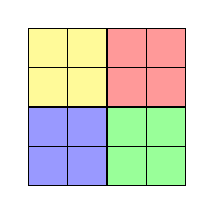
\begin{tikzpicture}[every node/.style={minimum size=.5cm-\pgflinewidth, outer sep=0pt}, scale=0.5]
    \fill[blue!40!white] (0,0) rectangle (2,2);
    \fill[red!40!white] (2,2) rectangle (4,4);
    \fill[green!40!white] (2,0) rectangle (4,2);
    \fill[yellow!40!white] (0,2) rectangle (2,4);
    \draw[step=1cm,color=black] (0,0) grid (4,4);
\end{tikzpicture}
\captionof{figure}{Tiled distribution}
\label{fig:dist-tiled}

% Rows 
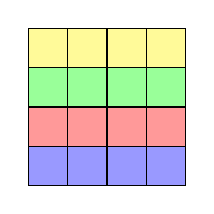
\begin{tikzpicture}[every node/.style={minimum size=.5cm-\pgflinewidth, outer sep=0pt}, scale=0.5]
    \fill[blue!40!white] (0,0) rectangle (4,1);
    \fill[red!40!white] (0,1) rectangle (4,2);
    \fill[green!40!white] (0,2) rectangle (4,3);
    \fill[yellow!40!white] (0,3) rectangle (4,4);
    \draw[step=1cm,color=black] (0,0) grid (4,4);
\end{tikzpicture}
\captionof{figure}{Rows distribution}
\label{fig:dist-rows}

\end{multicols}
\end{center}

A closely related consideration to the shape of the rank regions is what data
is shared between the ranks and when the data is shared.
\autoref{fig:cells-regions-and-halos} shows the halo regions which must be
shared between each rank every timestep. In the inital implementation \verb|MPI_Sendrecv|
was used to send these regions at the begining of each timestep. This is a
blocking operation, meaing the execution is blocked until the send and recieve
for that node have been completed. 

The results for this computation on 4 nodes using mpi compared to a serial
implementation are available in \autoref{}. This shows the relatively minor
improvement in performance even when the work is divided across the 4 nodes.
This is as a result of the blocking operations. At the begining of each
timestep each rank must wait for all the data to be send and for the ranks
above and below to send the halo regions. This can dramatically increase the
run times and result in idling time where the CPUs are just waiting for data to
be send.

\section{Non-Blocking Send}

MPI offers methods to avoid this wasted CPU time by enabling non-blocking
communication. This allows the CPU to asynchronously send and receive data
to and from a rank in the background, allowing the CPU to continue with other
computation in the meantime. The implementation of non-blocking sends in this
case required 3 MPI directives.

\begin{itemize}
    \item{\verb|MPI_Isend|}
    \item{\verb|MPI_Irecv|}
    \item{\verb|MPI_Wait|}
\end{itemize}

\verb|MPI_Isend| and \verb|MPI_Irecv| allow MPI to start sending and receiving
data respectively but does not wait for these operations to complete. An
\verb|MPI_Wait| is then required to ensure the data transfer has completed.
\autoref{algo:timestep} shows the implementation of each timestep. The key
difference between this implementation and the blocking one is the
communication. At the beginning of each timestep the send and receives are
initialised. Next the calculations for the inner cells, those which only depend
on cells stored in local memory, starts. This allows the cell transfer to take
place in the background whilst this computation is happening. After the inner
cells have been calculated an \verb|MPI_Wait| is used to ensure the
communication has finished. Finally the 2 outer rows are calculated using the
cells received during the communication.

This approach allows the majority of the communication to happen whilst the
others cells are being calculated. This dramatically reduces the wasted CPU
time, waiting for all the rank to be read and the communication to be
completed.
% RESULTS

\begin{algorithm}[H]

\SetAlgoLined
    Start receiving halo cells using \verb|MPI_Irecv|

    Start sending halo cells using \verb|MPI_Isend|

    \For{$i\gets1$ \KwTo $ny - 2$ \KwBy $1$}{
        Calculate next timestep cell values
    }

    Wait for alls sends and receives to be completed with \verb|MPI_Waitall|

    Calculate next timestep cell values for row 0 and ny - 1

 \caption{Timestep implementation}
 \label{algo:timestep}
\end{algorithm}


\begin{center}
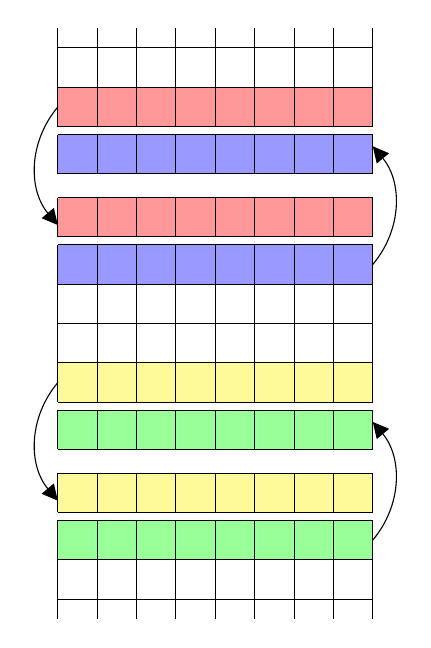
\begin{tikzpicture}[every node/.style={minimum size=.5cm-\pgflinewidth, outer sep=0pt}, scale=0.5]
    \fill[red!40!white, yshift=1cm] (0,6) rectangle (8,7);
    \draw[step=1cm,color=black,yshift=1cm] (0,6) grid (8,8.5);

    % Blue Halo
    \fill[blue!40!white, yshift=-0.2cm] (0,6) rectangle (8,7);
    \draw[step=1cm,color=black,yshift=-0.2cm] (0,6) grid (8,7);

    % Red Halo
    \fill[red!40!white, yshift=0.2cm] (0,4) rectangle (8,5);
    \draw[step=1cm,color=black,yshift=0.2cm] (0,4) grid (8,5);

    \fill[blue!40!white] (0,3) rectangle (8,4);
    \fill[yellow!40!white] (0,0) rectangle (8,1);
    \draw[step=1cm,color=black] (0,0) grid (8,4);

    % Green Halo
    \fill[green!40!white, yshift=-0.2cm] (0,0) rectangle (8,-1);
    \draw[step=1cm,color=black,yshift=-0.2cm] (0,0) grid (8,-1);
    
    % Yellow Halo
    \fill[yellow!40!white, yshift=0.2cm] (0,-2) rectangle (8,-3);
    \draw[step=1cm,color=black,yshift=0.2cm] (0,-2) grid (8,-3);

    \fill[green!40!white, yshift=-1cm] (0,-2) rectangle (8,-3);
    \draw[step=1cm,color=black,yshift=-1cm] (0,-2) grid (8,-4.5);

    % Arrows
    \draw [-{Triangle[length=2mm, width=2mm]}] (8, +3.5) to [bend right=40] (8, +6.5);
    \draw [-{Triangle[length=2mm, width=2mm]}] (0, +7.5) to [bend right=40] (0, +4.5);
    \draw [-{Triangle[length=2mm, width=2mm]}] (0, +0.5) to [bend right=40] (0, -2.5);
    \draw [-{Triangle[length=2mm, width=2mm]}] (8, -3.5) to [bend right=40] (8, -0.5);

\end{tikzpicture}
\captionof{figure}{Cell regions and halos}
\label{fig:cells-regions-and-halos}
\end{center}

% Inital implementation blocking send
% Data shape to reduce number of sends

\section{SOA vs AOS}

% Switching to AOS to ensure contigious data sends 
When sending data with MPI the data must be contiguous. This means the cells
being sent must either be stored in contiguous memory or be made contiguous
before the sends. However another consideration of performance is the
optimizations of individual nodes. Therefore if a data layout is good for the
MPI communication it may have the opposite effect on the overall performance.
The clearest example of this is with vectorisation.

\section{OpenMP MPI}

Although MPI uses distributed memory parallelism, which reduces run times by
sharing the workload across multiple CPUs, it is also important to optimize the
individual nodes. In this case it is possible to combine shared memory
parallelism, on each rank, with distributed memory parallelism. Using OpenMP
the loop for the inner cells in \autoref{algo:timestep} can be parallelised. This makes use of all the threads in each node resulting in a dramatic speed up.

% Results

This topic was discussed in more depth in the first report.

% Combining shared memory and distributed memory parallelism

\section{OpenCL}

\end{multicols}
\end{document}
